\documentclass[tikz,border=8pt]{standalone}
\usepackage{tikz}
\usepackage{xcolor}

\definecolor{cbgAcol}{RGB}{31,119,180}   % blue
\definecolor{cbgBcol}{RGB}{44,160,44}    % green
\definecolor{cbgCcol}{RGB}{230,159,0}    % orange
\definecolor{cbgDcol}{RGB}{142,68,173}   % purple
\definecolor{vtdcol}{RGB}{178,24,43}     % dark red
\definecolor{tractcol}{RGB}{20,20,20}

% helper: a legible label with an opaque white backdrop so crossing
% lines never make the text hard to read
\newcommand{\lbl}[4]{\node[#1, font=\bfseries\small, fill=white,
  fill opacity=0.88, text opacity=1, rounded corners=2pt, inner sep=2pt] at (#2,#3) {#4};}

\begin{document}
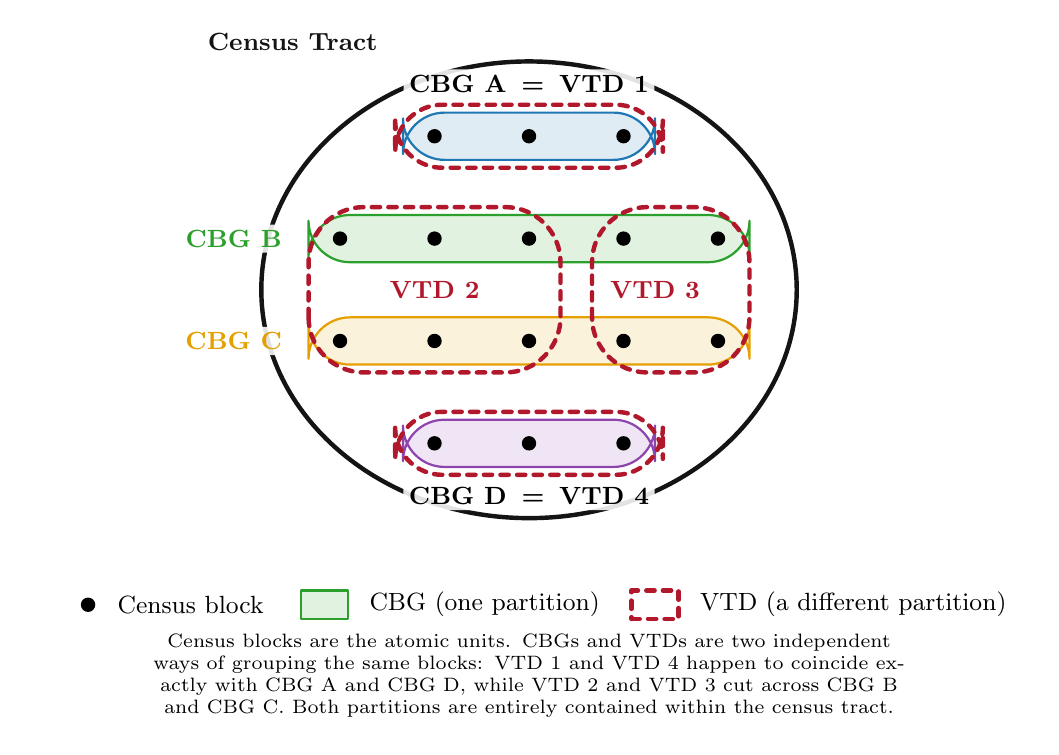
\begin{tikzpicture}[line cap=round, line join=round]

% ------------------------------------------------------------------
% Census tract: outer set, drawn as a true ellipse containing everything
% ------------------------------------------------------------------
\draw[tractcol, ultra thick] (0,0) ellipse [x radius=3.4, y radius=2.9];

% ------------------------------------------------------------------
% CBGs: four "slice" pills forming an oval partition of the blocks
% (top/bottom slices are short, middle two are long -> oval silhouette)
% ------------------------------------------------------------------
\draw[cbgAcol, thick, fill=cbgAcol!14, rounded corners=15pt]
  (-1.6,1.65) rectangle (1.6,2.25);                 % CBG A (top)
\draw[cbgBcol, thick, fill=cbgBcol!14, rounded corners=15pt]
  (-2.8,0.35) rectangle (2.8,0.95);                 % CBG B (upper-middle)
\draw[cbgCcol, thick, fill=cbgCcol!14, rounded corners=15pt]
  (-2.8,-0.95) rectangle (2.8,-0.35);                % CBG C (lower-middle)
\draw[cbgDcol, thick, fill=cbgDcol!14, rounded corners=15pt]
  (-1.6,-2.25) rectangle (1.6,-1.65);                % CBG D (bottom)

% ------------------------------------------------------------------
% VTDs: a *different* partition of the same blocks.
%  - VTD 1 coincides exactly with CBG A (drawn as a matching outline)
%  - VTD 4 coincides exactly with CBG D
%  - VTD 2 / VTD 3 cut vertically across CBG B and CBG C
% ------------------------------------------------------------------
\draw[vtdcol, ultra thick, dashed, rounded corners=17pt]
  (-1.7,1.55) rectangle (1.7,2.35);                  % VTD 1 = CBG A
\draw[vtdcol, ultra thick, dashed, rounded corners=17pt]
  (-1.7,-2.35) rectangle (1.7,-1.55);                % VTD 4 = CBG D
\draw[vtdcol, ultra thick, dashed, rounded corners=20pt]
  (-2.8,-1.05) rectangle (0.4,1.05);                 % VTD 2 (crosses B & C)
\draw[vtdcol, ultra thick, dashed, rounded corners=20pt]
  (0.8,-1.05) rectangle (2.8,1.05);                  % VTD 3 (crosses B & C)

% ------------------------------------------------------------------
% Census blocks (dots), arranged in an oval point cloud, drawn last
% so they sit on top of every boundary
% ------------------------------------------------------------------
\foreach \x in {-1.2,0,1.2}{ \fill[black] (\x,1.95) circle (2.6pt); }   % row A
\foreach \x in {-2.4,-1.2,0,1.2,2.4}{ \fill[black] (\x,0.65) circle (2.6pt); } % row B
\foreach \x in {-2.4,-1.2,0,1.2,2.4}{ \fill[black] (\x,-0.65) circle (2.6pt); } % row C
\foreach \x in {-1.2,0,1.2}{ \fill[black] (\x,-1.95) circle (2.6pt); }  % row D

% ------------------------------------------------------------------
% Labels (opaque backdrop keeps them readable over any crossing line)
% ------------------------------------------------------------------
\lbl{tractcol}{-3.0}{3.15}{Census Tract}
\lbl{black}{0}{2.62}{CBG A \,=\, VTD 1}
\lbl{black}{0}{-2.62}{CBG D \,=\, VTD 4}
\lbl{cbgBcol}{-3.75}{0.65}{CBG B}
\lbl{cbgCcol}{-3.75}{-0.65}{CBG C}
\lbl{vtdcol}{-1.2}{0}{VTD 2}
\lbl{vtdcol}{1.6}{0}{VTD 3}

% ------------------------------------------------------------------
% Legend
% ------------------------------------------------------------------
\begin{scope}[shift={(0,-4.0)}, font=\small]
  \fill[black] (-5.6,0) circle (2.6pt);
  \node[anchor=west] at (-5.35,0) {Census block};

  \draw[cbgBcol, thick, fill=cbgBcol!14] (-2.9,-0.18) rectangle (-2.3,0.18);
  \node[anchor=west] at (-2.15,0) {CBG (one partition)};

  \draw[vtdcol, ultra thick, dashed] (1.3,-0.18) -- (1.9,-0.18) -- (1.9,0.18) -- (1.3,0.18) -- cycle;
  \node[anchor=west] at (2.05,0) {VTD (a different partition)};
\end{scope}

\node[align=center, font=\scriptsize, text width=12.5cm] at (0, -4.9)
  {Census blocks are the atomic units. CBGs and VTDs are two independent ways
   of grouping the same blocks: VTD~1 and VTD~4 happen to coincide exactly
   with CBG~A and CBG~D, while VTD~2 and VTD~3 cut across CBG~B and CBG~C.
   Both partitions are entirely contained within the census tract.};

\end{tikzpicture}
\end{document}
